\section{Tree-Parzen Estimator}
%-----------------------------------------------------------------------
\begin{frame}[c]{Tree-Parzen Estimator}
\framesubtitle{Introduction}

\begin{itemize}
    \item Instead of modelling $
            P(\func \vert \dataset_{1:\bocount}) \propto P(\dataset_{1:\bocount} \vert \func) \times P(\func)$, TPE models $P(\dataset_{1:\bocount} \vert \func)$
    %\item \emph{Recall.} Bayesian optimization approach:
    %    \begin{equation*}
    %         P(\obs \vert \conf) \propto P(\conf \vert \obs) \times P(\obs)
    %    \end{equation*}
    \item TPE then defines two such distributions, $l$ and $g$:
        \begin{equation*}
            P(\conf \vert \obs) = 
                \begin{cases}
                    l(\conf) \text{ if } \obs < \obs^*\\
                    g(\conf) \text{ otherwise} 
                \end{cases}
        \end{equation*}
    where $\obs^*$ is an empirical threshold for a well-performing configuration (e.g., a $\gamma$ percentile of all observed $\obs$ in $D$)
    \item Distributions are approximated by kernel density estimators (Parzen estimators)
    \item Optimizing $l(\conf)/g(\conf)$ is equivalent to optimizing \emph{expected improvement} as the acquisition function in Bayesian optimization
    \item The \emph{tree} in the name is there because TPE can handle tree-structured search spaces 
        
\end{itemize}

\source{\href{https://papers.nips.cc/paper/4443-algorithms-for-hyper-parameter-optimization.pdf}{Bergstra et al. 2011}}

\end{frame}
%-----------------------------------------------------------------------
\begin{frame}[c]{Tree-Parzen Estimator}
\framesubtitle{Pseudocode}


\begin{center}
\begin{minipage}{0.75\textwidth}
\begin{algorithm}[H]
    %\DontPrintSemicolon
    \SetAlgoLined
    \setcounter{AlgoLine}{0}
    \SetKwInOut{Require}{Require}
    \SetKwInOut{Result}{Result}
    \Require{Search space $\pcs$, 
    		cost function $\cost$, 
    		\textcolor{blue}{percentile $\gamma$},
    		maximal number of function evaluations $\bobudget$}
    \Result{Best observed configuration $\conf$ according to $\iter[\bobudget]{\dataset}$}
    
    $\iter[0]{\dataset} \leftarrow \varnothing$\; 
    
    \For{$\bocount=1$ \KwTo $\bobudget$}{
		\textcolor{blue}{$\dataset_\text{good}, \dataset_\text{bad}$ $\leftarrow$ split $\iter[\bocount-1]{\dataset}$};\

        \textcolor{blue}{$l(\conf)$, $g(\conf)$ $\leftarrow$ fit KDE on $\dataset_\text{good}$, $\dataset_\text{bad}$ respectively};\

		\textcolor{blue}{$\pcs_\text{cand}$ $\leftarrow$ draw samples from $l$};\

		\textcolor{blue}{$\bonextsample \leftarrow \bonextsample \in \argmax_{\conf \in \pcs_\text{cand}} l(\conf) / g(\conf)$};\
		
		Query $\bonextobs$\;
		
		$\iter[\bocount]{\dataset} \leftarrow \iter[\bocount-1]{\dataset} \cup \{\langle \bonextsample, \bonextobs \rangle \}$\;
	}
    \caption{TPE loop}
\end{algorithm}
\end{minipage}
\end{center}

\source{Bergstra et al. 2011}

\end{frame}
%-----------------------------------------------------------------------
%-----------------------------------------------------------------------
\begin{frame}[c]{Tree-Parzen Estimator}
\framesubtitle{Example}
\onslide<1->
\begin{figure}
    \centering
    \only<1>{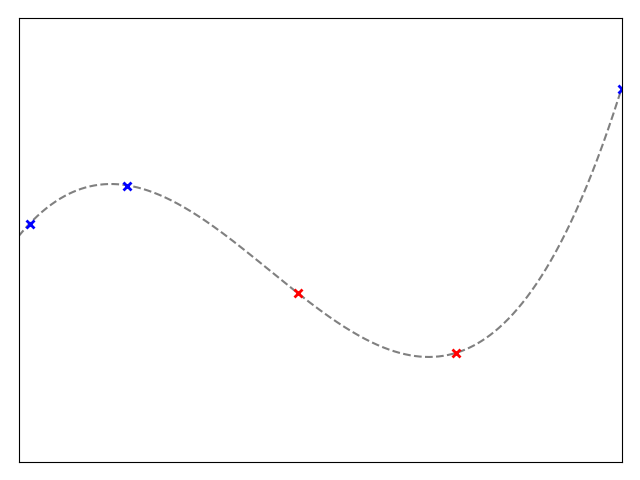
\includegraphics[width=0.6\textwidth]{w07_hpo_grey_box/images/tpe/tpeiter_1_observations.png}}
    \only<2>{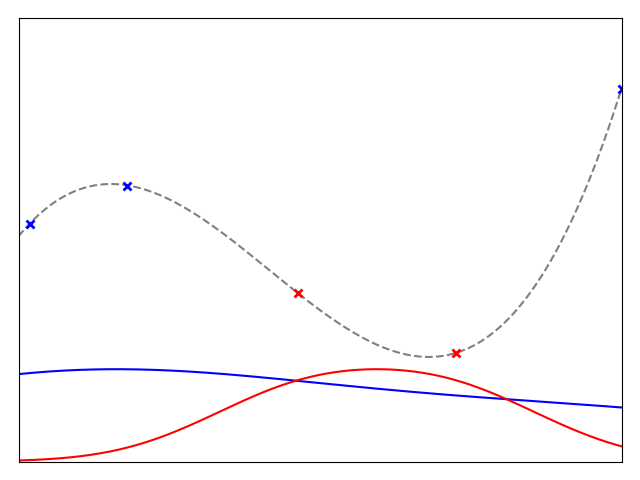
\includegraphics[width=0.6\textwidth]{w07_hpo_grey_box/images/tpe/tpeiter_1_pdfs.png}}
    \only<3>{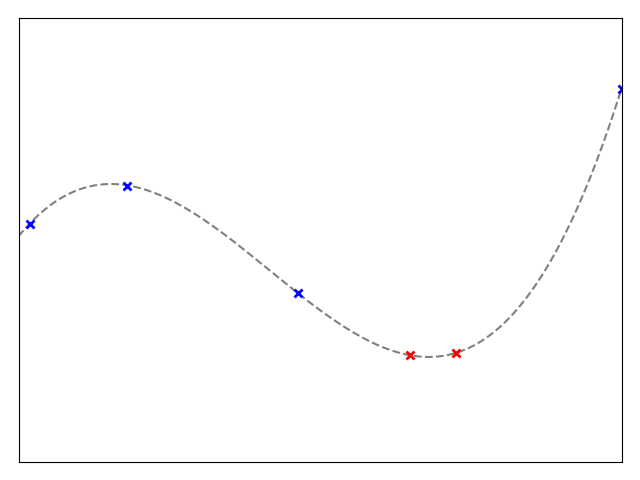
\includegraphics[width=0.6\textwidth]{w07_hpo_grey_box/images/tpe/tpeiter_2_observations.png}}
    \only<4>{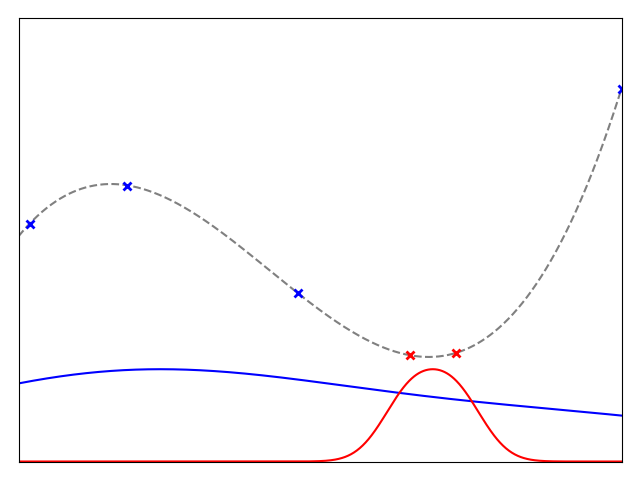
\includegraphics[width=0.6\textwidth]{w07_hpo_grey_box/images/tpe/tpeiter_2_pdfs.png}}
    \only<5>{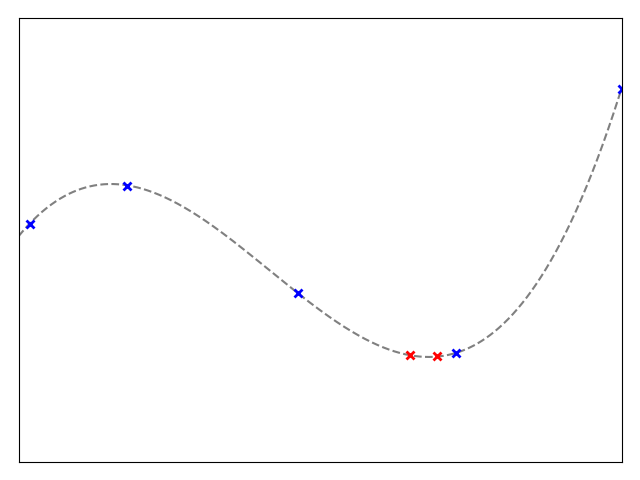
\includegraphics[width=0.6\textwidth]{w07_hpo_grey_box/images/tpe/tpeiter_3_observations.png}}
    \only<6>{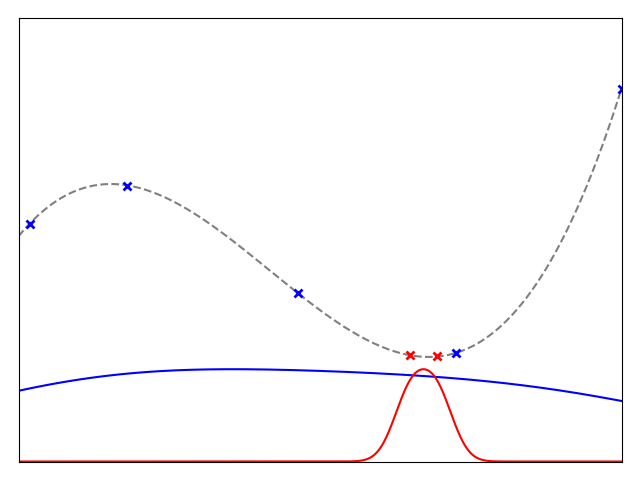
\includegraphics[width=0.6\textwidth]{w07_hpo_grey_box/images/tpe/tpeiter_3_pdfs.png}}
\end{figure}
\centering

\end{frame}
%-----------------------------------------------------------------------
\begin{frame}[c]{Tree-Parzen Estimator}
\framesubtitle{Further Details}

Remarks:

\begin{itemize}
	\item TPE models $p(\conf | \obs)$
	\begin{itemize}
		\item we can multiply it with a prior to add expert knowledge
	\end{itemize}
	\smallskip
	
	\pause
	
	\item Performance of TPE depends on:
	\begin{itemize}
		\item setting of $\gamma$ to trade-off exploration and exploitation
		\item bandwidth of the KDEs 
	\end{itemize}
	
	\pause
	
	\smallskip
	
	\smallskip
	\item A successful tool implementing TPE is \lit{\href{https://github.com/hyperopt/hyperopt}{hyperopt}}
\end{itemize}

\end{frame}
%-----------------------------------------------------------------------
\begin{frame}[c]{Tree-Parzen Estimator}
\framesubtitle{Summary}

\begin{columns}[T] % align columns
\begin{column}{.48\textwidth}
    \begin{block}{Advantages}
    \begin{itemize}
    	\item Efficient $O(N*d)$
    	\item Parallelizable
    	\item Robust
    	\item Deal with complex search spaces with priors
    \end{itemize}
    \end{block}
\end{column}%

\hfill%

\pause

\begin{column}{.48\textwidth}
    \begin{block}{Disadvantages}
    \begin{itemize}
    	\item Less sample-efficient than GPs
    \end{itemize}
    \end{block}
\end{column}
\end{columns}   

\end{frame}
%-----------------------------------------------------------------------
\begin{frame}[c]{Questions to Answer for Yourself / Discuss with Friends}

\begin{itemize}
    \item \emph{Discussion.} Is TPE really Bayesian optimization?
    \item \emph{Discussion.} How does $\gamma$ impact the optimization procedure?
    \item \emph{Repetition.} Derive that optimizing $l(\conf) / g(\conf)$ is equivalent to optimizing Expected Improvement.
\end{itemize}

\end{frame}